% ============================================================
% APÊNDICE A: ESPECIFICAÇÃO DOS CASOS DE USO
% ============================================================
\section*{APÊNDICE A: ESPECIFICAÇÃO DOS CASOS DE USO}
\addcontentsline{toc}{section}{APÊNDICE A: ESPECIFICAÇÃO DOS CASOS DE USO}

Esta seção apresenta a especificação textual detalhada dos oito casos de uso fundamentais que compõem o escopo operacional da plataforma WeFIND, descrevendo atores, pré-condições, fluxos principais, alternativas e exceções.

\vspace{0.5cm}

\subsection*{Caso de Uso UC01: Efetuar Login}
\noindent
\begin{table}[H]
\centering
\small
\begin{tabular}{|>{\raggedright\arraybackslash}p{3.2cm}|>{\raggedright\arraybackslash}p{11.8cm}|}
\hline
\textbf{Identificador} & UC01 \\ \hline
\textbf{Nome do Caso de Uso} & Efetuar Login \\ \hline
\textbf{Ator Principal} & Usuário Visitante \\ \hline
\textbf{Atores Secundários} & Serviço de Autenticação (Supabase Auth) e API do WhatsApp \\ \hline
\textbf{Resumo} & Permite ao usuário autenticar-se na plataforma mediante e-mail e senha, gerando token JWT de sessão persistente. \\ \hline
\textbf{Pré-Condições} & Possuir cadastro ativo no WeFIND. \\ \hline
\multicolumn{2}{|l|}{\textbf{Fluxo Principal:}} \\
\multicolumn{2}{|>{\raggedright\arraybackslash}p{15.4cm}|}{
1. O usuário aciona a opção ``Entrar'' na tela inicial.\par
2. O sistema exibe o formulário solicitando e-mail e senha.\par
3. O usuário preenche as credenciais e toca em ``Entrar''.\par
4. O sistema valida o formato sintático do e-mail e o comprimento da senha.\par
5. O sistema submete a requisição ao Supabase Auth.\par
6. O serviço valida as credenciais e confirma a validação da conta via WhatsApp.\par
7. O sistema armazena a sessão localmente (\textit{AsyncStorage}) e redireciona ao feed principal autenticado.
} \\ \hline
\multicolumn{2}{|l|}{\textbf{Fluxos Alternativos:}} \\
\multicolumn{2}{|>{\raggedright\arraybackslash}p{15.4cm}|}{
3a. Esquecimento de credenciais (\textit{<<extend>>}): o usuário aciona a opção \textbf{Redefinir Senha}, recebendo código OTP de 6 dígitos no WhatsApp para cadastro de nova senha.\par
1a. Exploração sem login: o usuário opta por ``Continuar explorando sem login'', acessando a visualização de publicações e do mapa em modo somente leitura.
} \\ \hline
\multicolumn{2}{|l|}{\textbf{Fluxos de Exceção:}} \\
\multicolumn{2}{|>{\raggedright\arraybackslash}p{15.4cm}|}{
4a. Campos obrigatórios vazios: o sistema impede o envio e exibe avisos de preenchimento obrigatório nos campos destacados.\par
6a. Credenciais incorretas: o sistema emite alerta visual de erro e retém o usuário no formulário para nova tentativa.
} \\ \hline
\textbf{Pós-Condições} & Sessão iniciada com permissões de publicação, chat e gestão de pets ativas. \\ \hline
\end{tabular}
\end{table}

\vspace{0.8cm}

\subsection*{Caso de Uso UC02: Realizar Cadastro}
\noindent
\begin{table}[H]
\centering
\small
\begin{tabular}{|>{\raggedright\arraybackslash}p{3.2cm}|>{\raggedright\arraybackslash}p{11.8cm}|}
\hline
\textbf{Identificador} & UC02 \\ \hline
\textbf{Nome do Caso de Uso} & Realizar Cadastro \\ \hline
\textbf{Ator Principal} & Usuário Visitante \\ \hline
\textbf{Atores Secundários} & Supabase Auth e Serviço de Mensageria (WhatsApp) \\ \hline
\textbf{Resumo} & Permite a novos membros criarem uma conta informando dados cadastrais e realizando a verificação por código de segurança no WhatsApp. \\ \hline
\textbf{Pré-Condições} & Dispositivo conectado à internet. \\ \hline
\multicolumn{2}{|l|}{\textbf{Fluxo Principal:}} \\
\multicolumn{2}{|>{\raggedright\arraybackslash}p{15.4cm}|}{
1. O usuário toca na opção ``Cadastre-se'' na tela de login.\par
2. O sistema abre o formulário de registro solicitando nome completo, e-mail, telefone WhatsApp e senha.\par
3. O usuário preenche as informações e confirma o cadastro.\par
4. O sistema valida os campos, cria o registro no Supabase Auth e aciona por inclusão (\textit{«include»}) o caso de uso \textbf{Verificar Código}, disparando um código OTP de 6 dígitos para o WhatsApp informado.\par
5. O sistema exibe a tela de confirmação de telefone com 6 campos numéricos.\par
6. O usuário digita o código recebido no WhatsApp.\par
7. O caso de uso \textbf{Verificar Código} valida a sequência numérica e ativa a conta de usuário permanentemente.
} \\ \hline
\multicolumn{2}{|l|}{\textbf{Fluxos Alternativos:}} \\
\multicolumn{2}{|>{\raggedright\arraybackslash}p{15.4cm}|}{
6a. Reenvio de código de segurança: caso não receba o código, o usuário aciona o botão de reenvio após o término da contagem regressiva do temporizador de segurança.
} \\ \hline
\multicolumn{2}{|l|}{\textbf{Fluxos de Exceção:}} \\
\multicolumn{2}{|>{\raggedright\arraybackslash}p{15.4cm}|}{
4a. E-mail ou telefone já cadastrados: o sistema emite alerta indicando a duplicidade cadastral e impede o registro repetido.\par
4b. Senha fora dos parâmetros: o sistema sinaliza que a senha deve possuir no mínimo 6 caracteres.\par
6b. Código incorreto ou expirado: o sistema sinaliza a inconsistência e solicita nova inserção.
} \\ \hline
\textbf{Pós-Condições} & Conta criada, validada em duas etapas e pronta para autenticação. \\ \hline
\end{tabular}
\end{table}

\clearpage

\subsection*{Caso de Uso UC03: Manter Publicação}
\noindent
\begin{table}[H]
\centering
\small
\begin{tabular}{|>{\raggedright\arraybackslash}p{3.2cm}|>{\raggedright\arraybackslash}p{11.8cm}|}
\hline
\textbf{Identificador} & UC03 \\ \hline
\textbf{Nome do Caso de Uso} & Manter Publicação \\ \hline
\textbf{Ator Principal} & Usuário (Autenticado) \\ \hline
\textbf{Atores Secundários} & Banco de Dados (PostgreSQL) e Supabase Storage \\ \hline
\textbf{Resumo} & Permite cadastrar, editar, alterar status (localizado/adotado) ou excluir anúncios de animais perdidos, encontrados ou para adoção. \\ \hline
\textbf{Pré-Condições} & Usuário autenticado e com permissão de localização ativa. \\ \hline
\multicolumn{2}{|l|}{\textbf{Fluxo Principal:}} \\
\multicolumn{2}{|>{\raggedright\arraybackslash}p{15.4cm}|}{
1. O usuário aciona o botão de nova publicação (``+'') na barra de navegação.\par
2. O sistema apresenta o formulário solicitando a categoria: ``Perdido'', ``Encontrado'' ou ``Adoção''.\par
3. O usuário seleciona a categoria. No caso de animal encontrado, define se foi ``Visto na rua'' ou se ``Está em Lar Temporário''.\par
4. O usuário adiciona fotografias (com recorte integrado) e seleciona os atributos físicos do pet (espécie, raça, porte, cor, idade).\par
5. O sistema executa obrigatoriamente por inclusão (\textit{<<include>>}) o caso de uso \textbf{Selecionar Localização no Mapa}, capturando as coordenadas geográficas.\par
6. O usuário confirma a publicação.\par
7. O sistema envia as fotos ao Storage e grava os dados na tabela \textit{items}.\par
8. A publicação passa a ser exibida no feed e no mapa para a comunidade.
} \\ \hline
\multicolumn{2}{|l|}{\textbf{Fluxos Alternativos:}} \\
\multicolumn{2}{|>{\raggedright\arraybackslash}p{15.4cm}|}{
3a. Informar tutor de terceiros (\textit{<<extend>>}): o usuário aciona a extensão para indicar o contato de outro responsável pelo animal.\par
4a. Edição de publicação existente: o autor atualiza fotos ou descrições do anúncio já publicado.\par
4b. Encerramento com sucesso: o autor altera o status para ``Reencontrado'' ou ``Adotado'', arquivando a publicação.
} \\ \hline
\multicolumn{2}{|l|}{\textbf{Fluxos de Exceção:}} \\
\multicolumn{2}{|>{\raggedright\arraybackslash}p{15.4cm}|}{
4c. Imagem inválida ou tamanho excessivo: o sistema impede o upload e solicita a seleção de uma foto válida.\par
5a. Ponto no mapa não demarcado: o sistema bloqueia a submissão e exige a marcação das coordenadas geográficas.
} \\ \hline
\textbf{Pós-Condições} & Publicação persistida, visível no mapa e disponível para a comunidade. \\ \hline
\end{tabular}
\end{table}

\vspace{0.8cm}

\subsection*{Caso de Uso UC04: Registrar Avistamento}
\noindent
\begin{table}[H]
\centering
\small
\begin{tabular}{|>{\raggedright\arraybackslash}p{3.2cm}|>{\raggedright\arraybackslash}p{11.8cm}|}
\hline
\textbf{Identificador} & UC04 \\ \hline
\textbf{Nome do Caso de Uso} & Registrar Avistamento \\ \hline
\textbf{Ator Principal} & Usuário (Autenticado) \\ \hline
\textbf{Atores Secundários} & Banco de Dados (PostgreSQL) e Serviço de Notificações \\ \hline
\textbf{Resumo} & Permite a um membro da comunidade informar novas coordenadas e fotos do local onde viu um animal perdido na rua, atualizando o rastro de busca. \\ \hline
\textbf{Pré-Condições} & O animal deve estar publicado com status ``Perdido''. \\ \hline
\multicolumn{2}{|l|}{\textbf{Fluxo Principal:}} \\
\multicolumn{2}{|>{\raggedright\arraybackslash}p{15.4cm}|}{
1. Ao visualizar os detalhes de um animal perdido, o usuário aciona a opção ``Vi esse Pet''.\par
2. O sistema abre o modal de avistamento solicitando foto do local e relato.\par
3. O usuário captura ou anexa uma fotografia do animal avistado.\par
4. O sistema inclui obrigatoriamente (\textit{<<include>>}) o caso de uso \textbf{Selecionar Localização no Mapa}, capturando o ponto GPS do avistamento.\par
5. O usuário confirma o envio do avistamento.\par
6. O sistema atualiza atomicamente o marcador principal do animal para as novas coordenadas e grava o histórico em \textit{item\_sightings}.\par
7. O sistema dispara notificação push imediata ao tutor do pet informando a nova localização.
} \\ \hline
\multicolumn{2}{|l|}{\textbf{Fluxos Alternativos:}} \\
\multicolumn{2}{|>{\raggedright\arraybackslash}p{15.4cm}|}{
4a. Ajuste manual de localização: caso o sinal de GPS esteja impreciso, o usuário arrasta manualmente o pino até o local visualizado na rua.
} \\ \hline
\multicolumn{2}{|l|}{\textbf{Fluxos de Exceção:}} \\
\multicolumn{2}{|>{\raggedright\arraybackslash}p{15.4cm}|}{
4b. Coordenadas geográficas ausentes: o sistema impede a gravação do avistamento enquanto o ponto no mapa não for confirmado.\par
5a. Falha temporária de rede: o sistema retém os dados digitados e sugere nova tentativa de envio.
} \\ \hline
\textbf{Pós-Condições} & Marcador do animal reposicionado no mapa, tutor alertado e histórico de rastro atualizado. \\ \hline
\end{tabular}
\end{table}

\clearpage

\subsection*{Caso de Uso UC05: Enviar Mensagem}
\noindent
\begin{table}[H]
\centering
\small
\begin{tabular}{|>{\raggedright\arraybackslash}p{3.2cm}|>{\raggedright\arraybackslash}p{11.8cm}|}
\hline
\textbf{Identificador} & UC05 \\ \hline
\textbf{Nome do Caso de Uso} & Enviar Mensagem \\ \hline
\textbf{Ator Principal} & Usuário (Autenticado) \\ \hline
\textbf{Atores Secundários} & Serviço de Mensagens em Tempo Real (Supabase WebSockets) \\ \hline
\textbf{Resumo} & Viabiliza canal direto e privativo de troca de mensagens e imagens entre o tutor do animal e voluntários da comunidade sem expor contatos telefônicos. \\ \hline
\textbf{Pré-Condições} & Ambos os usuários devem possuir cadastro ativo. \\ \hline
\multicolumn{2}{|l|}{\textbf{Fluxo Principal:}} \\
\multicolumn{2}{|>{\raggedright\arraybackslash}p{15.4cm}|}{
1. Na tela de detalhes da publicação, o usuário aciona o botão ``Entrar em Contato''.\par
2. O sistema cria ou recupera a sala de conversa existente entre os dois usuários para aquele animal.\par
3. O sistema abre a interface de chat em tempo real.\par
4. O usuário digita a mensagem ou anexa uma foto e confirma o envio.\par
5. O sistema transmite a mensagem via WebSockets e notifica o destinatário via notificação push.\par
6. A mensagem é persistida na tabela \textit{messages} e exibida na conversa.
} \\ \hline
\multicolumn{2}{|l|}{\textbf{Fluxos Alternativos:}} \\
\multicolumn{2}{|>{\raggedright\arraybackslash}p{15.4cm}|}{
5a. Destinatário offline: a mensagem é gravada de modo permanente no banco de dados e sincronizada assim que o destinatário abrir o aplicativo.
} \\ \hline
\multicolumn{2}{|l|}{\textbf{Fluxos de Exceção:}} \\
\multicolumn{2}{|>{\raggedright\arraybackslash}p{15.4cm}|}{
1a. Tentativa de contato consigo mesmo: o sistema oculta a opção de chat quando o visualizador é o próprio autor do anúncio.\par
4a. Mensagem vazia: o sistema desabilita o botão de envio enquanto não houver conteúdo textual ou anexo de mídia.
} \\ \hline
\textbf{Pós-Condições} & Canal de comunicação estabelecido com histórico mantido na caixa de entrada. \\ \hline
\end{tabular}
\end{table}

\vspace{0.8cm}

\subsection*{Caso de Uso UC06: Compartilhar Publicação}
\noindent
\begin{table}[H]
\centering
\small
\begin{tabular}{|>{\raggedright\arraybackslash}p{3.2cm}|>{\raggedright\arraybackslash}p{11.8cm}|}
\hline
\textbf{Identificador} & UC06 \\ \hline
\textbf{Nome do Caso de Uso} & Compartilhar Publicação \\ \hline
\textbf{Ator Principal} & Usuário / Usuário Visitante \\ \hline
\textbf{Atores Secundários} & Módulo Gerador de Código QR e API Nativa de Compartilhamento \\ \hline
\textbf{Resumo} & Permite a qualquer usuário renderizar automaticamente artes gráficas diagramadas em múltiplos formatos (A4, Stories e Feed) contendo código QR para divulgação rápida. \\ \hline
\textbf{Pré-Condições} & O animal deve possuir ao menos uma fotografia cadastrada. \\ \hline
\multicolumn{2}{|l|}{\textbf{Fluxo Principal:}} \\
\multicolumn{2}{|>{\raggedright\arraybackslash}p{15.4cm}|}{
1. Na tela de detalhes da publicação, o usuário clica em ``Compartilhar Cartaz''.\par
2. O sistema abre o modal com pré-visualização ao vivo da arte gerada.\par
3. O sistema gera dinamicamente o código QR apontando para o link público do animal.\par
4. O usuário seleciona o formato desejado (A4 para impressão, Stories 9:16 ou Feed 1:1).\par
5. O usuário escolhe entre salvar a imagem na galeria ou acionar o compartilhamento direto via WhatsApp ou redes sociais.\par
6. O sistema exporta o arquivo de imagem em alta definição.
} \\ \hline
\multicolumn{2}{|l|}{\textbf{Fluxos Alternativos:}} \\
\multicolumn{2}{|>{\raggedright\arraybackslash}p{15.4cm}|}{
4a. Cópia de texto rápido: o sistema oferece botão auxiliar para copiar texto formatado contendo os dados essenciais e o link web do animal para colar em conversas.
} \\ \hline
\multicolumn{2}{|l|}{\textbf{Fluxos de Exceção:}} \\
\multicolumn{2}{|>{\raggedright\arraybackslash}p{15.4cm}|}{
1a. Ausência de fotografias: o sistema informa que é obrigatório dispor de pelo menos uma foto para diagramar o cartaz de busca.
} \\ \hline
\textbf{Pós-Condições} & Peça gráfica diagramada e compartilhada nos canais comunitários. \\ \hline
\end{tabular}
\end{table}

\clearpage

\subsection*{Caso de Uso UC07: Cadastro Preventivo de Pets}
\noindent
\begin{table}[H]
\centering
\small
\begin{tabular}{|>{\raggedright\arraybackslash}p{3.2cm}|>{\raggedright\arraybackslash}p{11.8cm}|}
\hline
\textbf{Identificador} & UC07 \\ \hline
\textbf{Nome do Caso de Uso} & Cadastro Preventivo de Pets \\ \hline
\textbf{Ator Principal} & Usuário (Autenticado) \\ \hline
\textbf{Atores Secundários} & Banco de Dados (PostgreSQL) e Supabase Storage \\ \hline
\textbf{Resumo} & Permite cadastrar previamente os dados dos animais domésticos tutelados, gerando a ficha de identificação com código QR de autenticidade. \\ \hline
\textbf{Pré-Condições} & Usuário logado na sua conta. \\ \hline
\multicolumn{2}{|l|}{\textbf{Fluxo Principal:}} \\
\multicolumn{2}{|>{\raggedright\arraybackslash}p{15.4cm}|}{
1. O usuário acessa a opção ``Animais Tutelados'' no menu do perfil.\par
2. O sistema lista os animais tutelados previamente cadastrados ou oferece a opção de novo cadastro.\par
3. O usuário insere a foto do animal, nome, espécie, raça, data de nascimento e dados veterinários (vacinas e castração).\par
4. O usuário confirma o salvamento dos dados.\par
5. O sistema grava os registros e gera a ficha de identificação do animal tutelado com código QR e identificador único.\par
6. A ficha do animal fica disponível para consulta, emissão da carteirinha ou acionamento de alerta de desaparecimento.
} \\ \hline
\multicolumn{2}{|l|}{\textbf{Fluxos Alternativos:}} \\
\multicolumn{2}{|>{\raggedright\arraybackslash}p{15.4cm}|}{
6a. Acionamento de alerta de desaparecimento: caso o animal tutelado desapareça ou fuja, o tutor aciona o comando de alerta de desaparecimento, transformando a ficha preventiva diretamente em uma publicação de busca no mapa sem necessidade de redigitação.
} \\ \hline
\multicolumn{2}{|l|}{\textbf{Fluxos de Exceção:}} \\
\multicolumn{2}{|>{\raggedright\arraybackslash}p{15.4cm}|}{
3a. Campos obrigatórios em branco: o sistema barra a finalização do registro caso nome ou espécie do pet não tenham sido informados.
} \\ \hline
\textbf{Pós-Condições} & Cadastro do animal tutelado ativo e vinculado à conta do tutor. \\ \hline
\end{tabular}
\end{table}

\vspace{0.8cm}

\subsection*{Caso de Uso UC08: Manter Moderação e Denúncias}
\noindent
\begin{table}[H]
\centering
\small
\begin{tabular}{|>{\raggedright\arraybackslash}p{3.2cm}|>{\raggedright\arraybackslash}p{11.8cm}|}
\hline
\textbf{Identificador} & UC08 \\ \hline
\textbf{Nome do Caso de Uso} & Manter Moderação e Denúncias \\ \hline
\textbf{Ator Principal} & Administrador \\ \hline
\textbf{Atores Secundários} & Banco de Dados (PostgreSQL) \\ \hline
\textbf{Resumo} & Permite ao administrador inspecionar relatórios de denúncia enviados pela comunidade sobre anúncios indevidos, aplicando sanções ou exclusão do conteúdo. \\ \hline
\textbf{Pré-Condições} & Conta autenticada com perfil de administrador (\textit{isAdmin = true}). \\ \hline
\multicolumn{2}{|l|}{\textbf{Fluxo Principal:}} \\
\multicolumn{2}{|>{\raggedright\arraybackslash}p{15.4cm}|}{
1. O administrador acessa a tela de moderação do sistema.\par
2. O sistema lista os anúncios que receberam denúncias dos usuários com o respectivo motivo.\par
3. O administrador examina as fotos, o texto e os dados do anúncio reportado.\par
4. O administrador seleciona a ação cabível: desconsiderar denúncia, suspender anúncio ou excluir publicação.\par
5. O sistema atualiza o status do anúncio e registra a decisão no log de auditoria.
} \\ \hline
\multicolumn{2}{|l|}{\textbf{Fluxos Alternativos:}} \\
\multicolumn{2}{|>{\raggedright\arraybackslash}p{15.4cm}|}{
4a. Descarte de denúncia infundada: o administrador constata a conformidade do anúncio e arquiva o chamado mantendo a publicação ativa.\par
4b. Solicitação de ajuste: o administrador suspende temporariamente o anúncio e solicita alterações de dados ao usuário.
} \\ \hline
\multicolumn{2}{|l|}{\textbf{Fluxos de Exceção:}} \\
\multicolumn{2}{|>{\raggedright\arraybackslash}p{15.4cm}|}{
4c. Infração grave ou fraude dolosa: o administrador exclui o anúncio e suspende preventivamente a conta do usuário infrator.
} \\ \hline
\textbf{Pós-Condições} & Publicação moderada e integridade comunitária da plataforma assegurada. \\ \hline
\end{tabular}
\end{table}

\clearpage

% ============================================================
% APÊNDICE B: INSTRUMENTOS DE PESQUISA
% ============================================================
\section*{APÊNDICE B: INSTRUMENTOS DE PESQUISA (QUESTIONÁRIO DE CAMPO E ESCALA SUS)}
\addcontentsline{toc}{section}{APÊNDICE B: INSTRUMENTOS DE PESQUISA (QUESTIONÁRIO DE CAMPO E ESCALA SUS)}

Este apêndice documenta os instrumentos de coleta de dados primários aplicados durante a pesquisa prática inicial com tutores (Google Forms) e durante os testes práticos de validação da aplicação (Escala SUS).

\vspace{0.4cm}
\subsection*{B.1 Questionário de Levantamento de Campo com Tutores}

Instrumento estruturado de coleta de dados primários aplicado aos 20 participantes voluntários (tutores de animais domésticos, protetores independentes e pessoas engajadas na causa animal) durante a etapa de diagnóstico e levantamento de requisitos (Capítulo 3).

\vspace{0.3cm}
\noindent
\textbf{Instruções ao participante:} Este questionário tem como finalidade diagnosticar os hábitos de identificação animal e as principais dificuldades enfrentadas durante o desaparecimento e resgate de animais de estimação (incluindo cães, gatos, aves e outros animais domésticos). Por favor, responda a cada uma das questões a seguir:

\vspace{0.4cm}
\noindent
\textbf{Questão 1: Seu(s) animal(is) de estimação possui(em) microchip de identificação eletrônica?}\par
[ ] Sim\par
[ ] Não\par
[ ] Não sei informar

\vspace{0.3cm}
\noindent
\textbf{Questão 2: Seu(s) animal(is) de estimação utiliza(m) algum tipo de coleira ou plaquinha de identificação?}\par
[ ] Não utiliza nenhum tipo de coleira\par
[ ] Sim, coleira com plaquinha de identificação visual (nome e telefone)\par
[ ] Sim, coleira equipada com dispositivo GPS ou rastreamento eletrônico

\vspace{0.3cm}
\noindent
\textbf{Questão 3: Algum animal de estimação seu já fugiu ou você já auxiliou no resgate de um animal perdido?}\par
[ ] Sim, meu animal de estimação já desapareceu\par
[ ] Já auxiliei no resgate ou localização de animal de terceiro\par
[ ] Ambas as situações anteriores\par
[ ] Nenhuma das opções

\vspace{0.3cm}
\noindent
\textbf{Questão 4: Quais canais você mais costuma utilizar para divulgar um animal perdido?}\par
[ ] Redes sociais (Instagram e Facebook)\par
[ ] Grupos de troca de mensagens no WhatsApp\par
[ ] Cartazes impressos afixados em postes e comércios\par
[ ] Contato presencial com vizinhos da localidade\par
[ ] Comunicação a clínicas veterinárias locais

\vspace{0.3cm}
\noindent
\textbf{Questão 5: Quais as maiores dificuldades encontradas na divulgação tradicional?}\par
\textit{Campo discursivo aberto para relatos dos tutores sobre demora na disseminação, perda de alcance em feeds, falta de mapas e receio de golpes ao divulgar telefone pessoal.}

\vspace{0.3cm}
\noindent
\textbf{Questão 6: Em uma escala de 1 a 5, qual o nível de utilidade de visualizar animais perdidos em um mapa interativo com filtro de proximidade?}\par
[ ] 1 (Sem utilidade)\par
[ ] 2 (Pouca utilidade)\par
[ ] 3 (Utilidade moderada)\par
[ ] 4 (Muita utilidade)\par
[ ] 5 (Extrema utilidade)

\vspace{0.3cm}
\noindent
\textbf{Questão 7: Você utilizaria um aplicativo comunitário gratuito dedicado exclusivamente ao resgate e divulgação de animais?}\par
[ ] Sim, certamente\par
[ ] Provavelmente sim\par
[ ] Não tenho interesse

\vspace{0.3cm}
\noindent
\textbf{Questão 8: Quais recursos você consideraria mais importantes em um aplicativo como o WeFIND?}\par
[ ] Geração automática de cartazes de busca com código QR\par
[ ] Bate-papo privativo em tempo real para contato seguro\par
[ ] Cadastro preventivo e identificação de animais tutelados\par
[ ] Filtros avançados por espécie (cães, gatos, aves e outros), cor e porte do animal\par
[ ] Mural comunitário com relatos e fotos de reencontros felizes

\vspace{0.6cm}

\subsection*{B.2 Questionário de Avaliação de Usabilidade (Escala SUS)}

Instrumento padronizado de avaliação de usabilidade aplicado aos 20 voluntários participantes dos testes práticos da aplicação desenvolvida (Capítulo 8), elaborado segundo a metodologia padronizada \textit{System Usability Scale} (LEWIS, 2021; SAURO; LEWIS, 2022). 

\vspace{0.3cm}
\noindent
\textbf{Instruções ao participante:} Para cada uma das afirmações a seguir, assinale com um ``X'' o nível de concordância que melhor representa sua experiência prática com o aplicativo WeFIND, em uma escala de 1 (\textbf{Discordo Totalmente}, DT) a 5 (\textbf{Concordo Totalmente}, CT):

\vspace{0.5cm}
\begin{table}[H]
\centering
\small
\begin{tabular}{|c|>{\raggedright\arraybackslash}p{8.8cm}|c|c|c|c|c|}
\hline
\textbf{Nº} & \textbf{Afirmação Avaliada} & \textbf{1 (DT)} & \textbf{2} & \textbf{3} & \textbf{4} & \textbf{5 (CT)} \\ \hline
1 & Eu acho que gostaria de utilizar o WeFIND com frequência em situações de busca. & [ ] & [ ] & [ ] & [ ] & [ ] \\ \hline
2 & Eu achei o aplicativo desnecessariamente complexo. & [ ] & [ ] & [ ] & [ ] & [ ] \\ \hline
3 & Eu achei o sistema fácil e intuitivo de utilizar. & [ ] & [ ] & [ ] & [ ] & [ ] \\ \hline
4 & Eu acho que precisaria do suporte de uma pessoa técnica para conseguir utilizar o aplicativo. & [ ] & [ ] & [ ] & [ ] & [ ] \\ \hline
5 & Eu achei que as várias funções do sistema estavam muito bem integradas. & [ ] & [ ] & [ ] & [ ] & [ ] \\ \hline
6 & Eu achei que havia muita inconsistência neste sistema. & [ ] & [ ] & [ ] & [ ] & [ ] \\ \hline
7 & Eu imagino que a maioria das pessoas aprenderia a utilizar este aplicativo muito rapidamente. & [ ] & [ ] & [ ] & [ ] & [ ] \\ \hline
8 & Eu achei o aplicativo muito incômodo ou complicado de utilizar. & [ ] & [ ] & [ ] & [ ] & [ ] \\ \hline
9 & Eu me senti muito confiante e seguro utilizando o aplicativo. & [ ] & [ ] & [ ] & [ ] & [ ] \\ \hline
10 & Eu precisei aprender muitas coisas novas antes de conseguir utilizar o sistema. & [ ] & [ ] & [ ] & [ ] & [ ] \\ \hline
\end{tabular}
\end{table}

\clearpage

% ============================================================
% APÊNDICE C: GUIA DE UTILIZAÇÃO (MANUAL DO USUÁRIO)
% ============================================================
\section*{APÊNDICE C: GUIA DE UTILIZAÇÃO DO SISTEMA WeFIND (MANUAL DO USUÁRIO)}
\addcontentsline{toc}{section}{APÊNDICE C: GUIA DE UTILIZAÇÃO DO SISTEMA WeFIND (MANUAL DO USUÁRIO)}

Este guia orienta tutores e voluntários na utilização prática do aplicativo WeFIND, detalhando as operações centrais passo a passo através de capturas de tela do sistema.

\vspace{0.4cm}

\subsection*{Passo 1: Autenticação e Criação de Conta}
\noindent
Ao abrir o aplicativo, o usuário visualiza a tela de login. Caso ainda não possua cadastro, basta tocar em \textbf{``Cadastre-se''} para registrar seu perfil com nome, e-mail e telefone WhatsApp. A Figura C1 apresenta as telas de acesso e cadastro.

\vspace{0.2cm}
\noindent\begin{minipage}{\linewidth}
\centering
    \textbf{Figura C1: Telas de Login e Cadastro de Usuário}\\[0.2cm]
    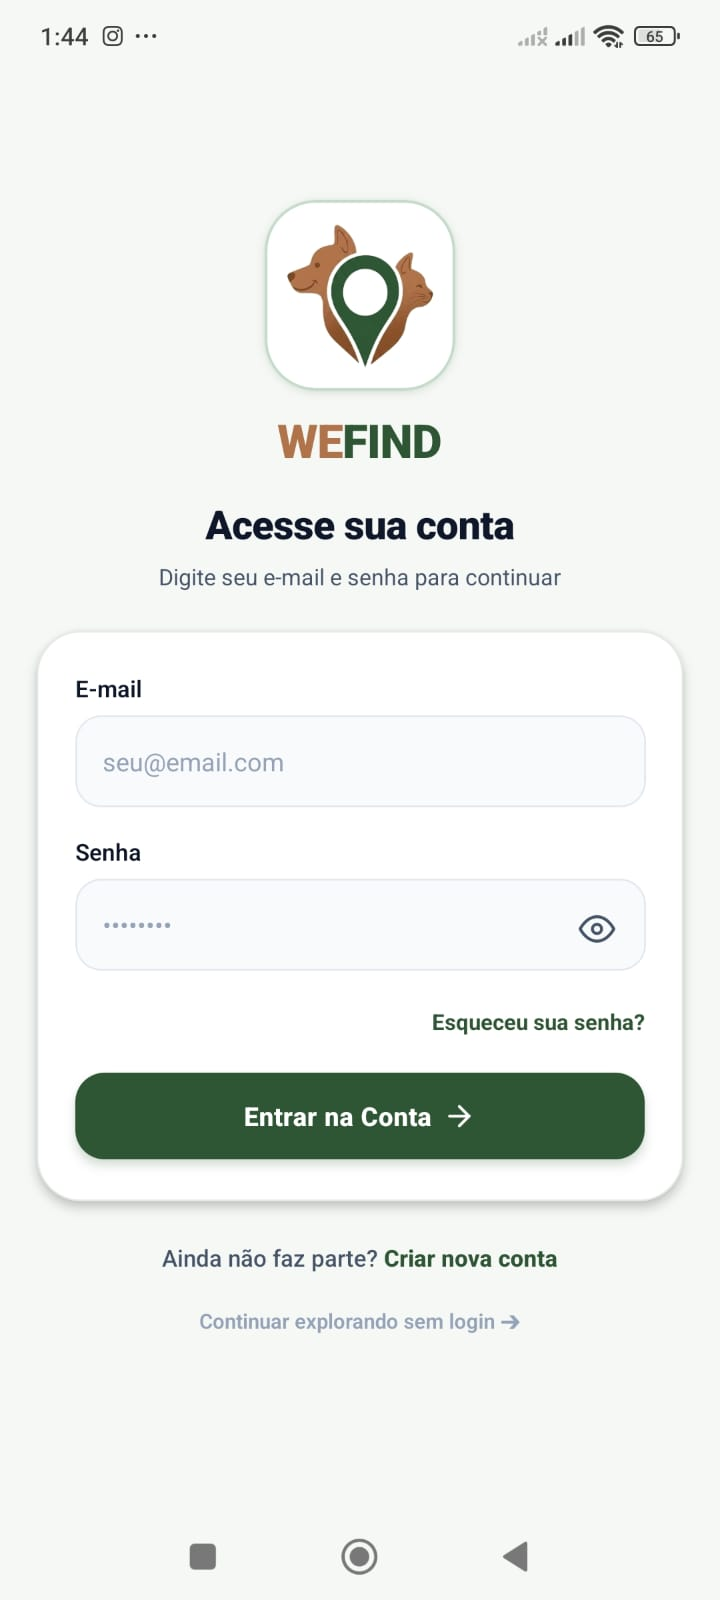
\includegraphics[height=7.8cm, keepaspectratio]{imagens/05_manual_usuario/figura15_tela_login.jpeg}
    \hspace{0.5cm}
    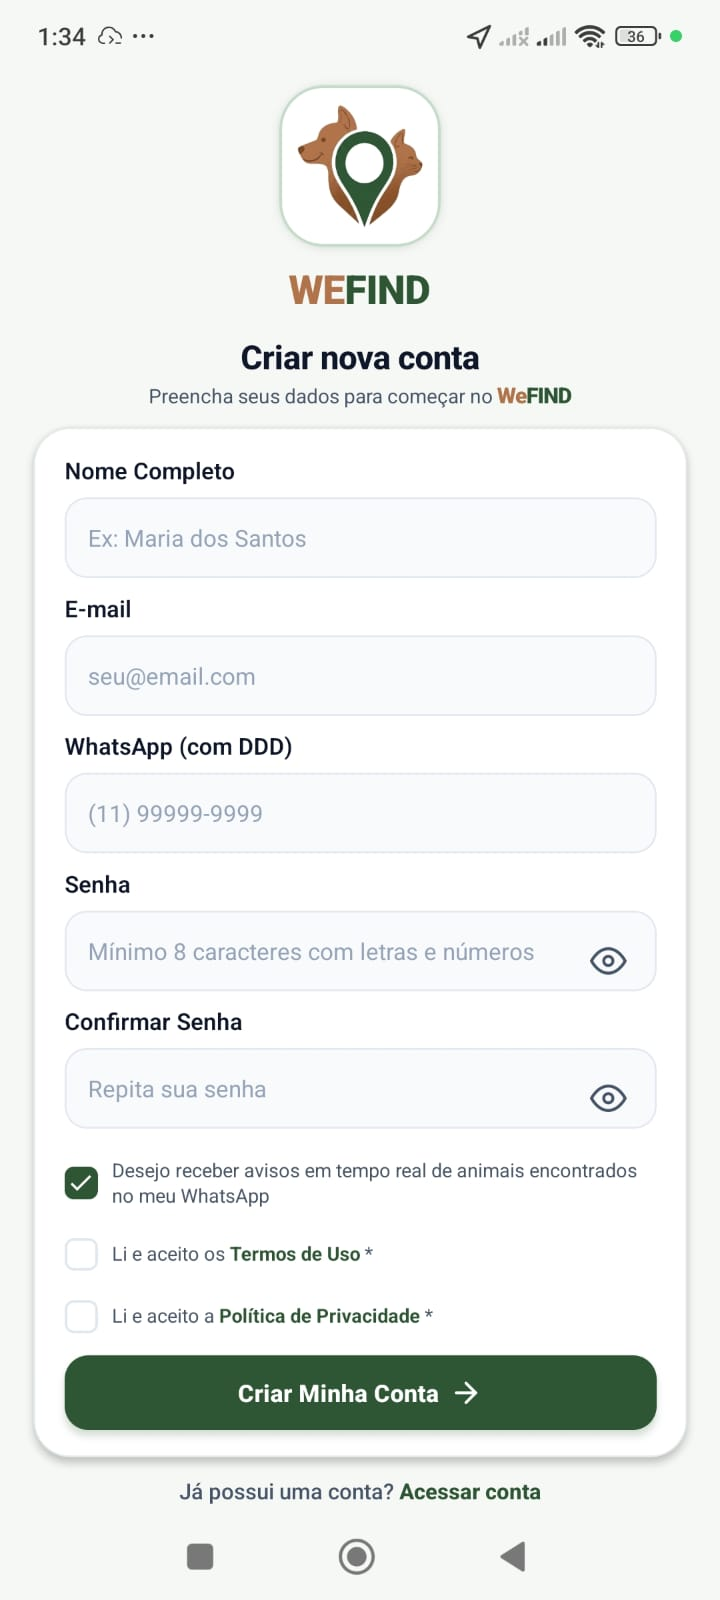
\includegraphics[height=7.8cm, keepaspectratio]{imagens/04_telas_aplicativo/tela-criar-conta.jpeg}\\[0.15cm]
    \begin{tabular}{p{5.0cm} p{5.0cm}}
        \centering\footnotesize (a) Tela de Login & \centering\footnotesize (b) Tela de Cadastro
    \end{tabular}\\[0.15cm]
    {\footnotesize Fonte: Autoria própria (2026)}
\end{minipage}

\clearpage

\subsection*{Passo 2: Navegação no Mapa Interativo e Traçado de Rotas}
\noindent
Após o acesso, o usuário explora as publicações no feed ordenado por proximidade e no mapa georreferenciado por GPS, podendo filtrar os animais por espécie, porte ou raio de distância e traçar rotas de deslocamento em tempo real até o animal avistado. A Figura C2 ilustra o mapa interativo e o traçado de rota.

\vspace{0.2cm}
\noindent\begin{minipage}{\linewidth}
\centering
    \textbf{Figura C2: Telas de Mapa Interativo e Traçado de Rota até o Animal}\\[0.2cm]
    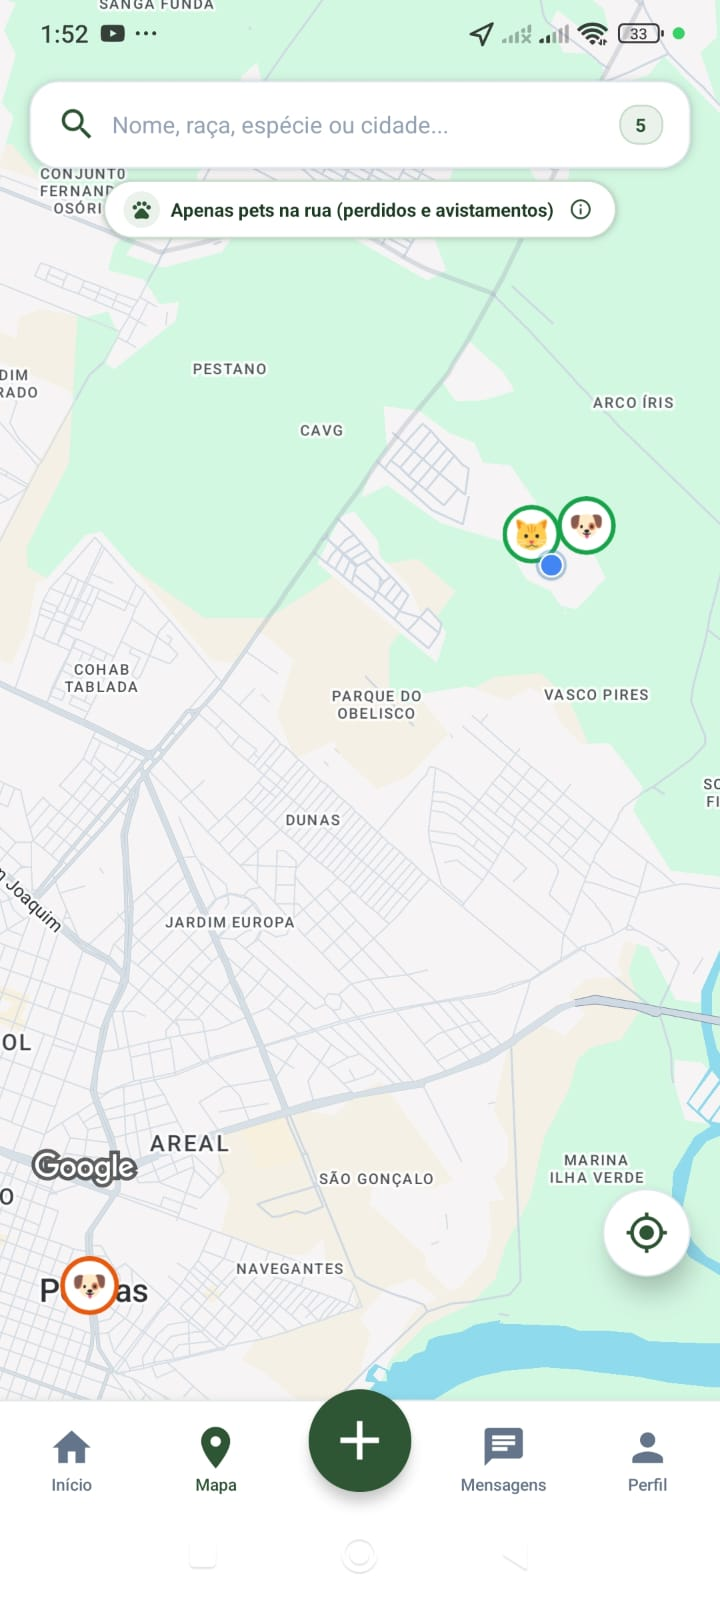
\includegraphics[height=7.8cm, keepaspectratio]{imagens/04_telas_aplicativo/tela-mapa-principal.jpeg}
    \hspace{0.5cm}
    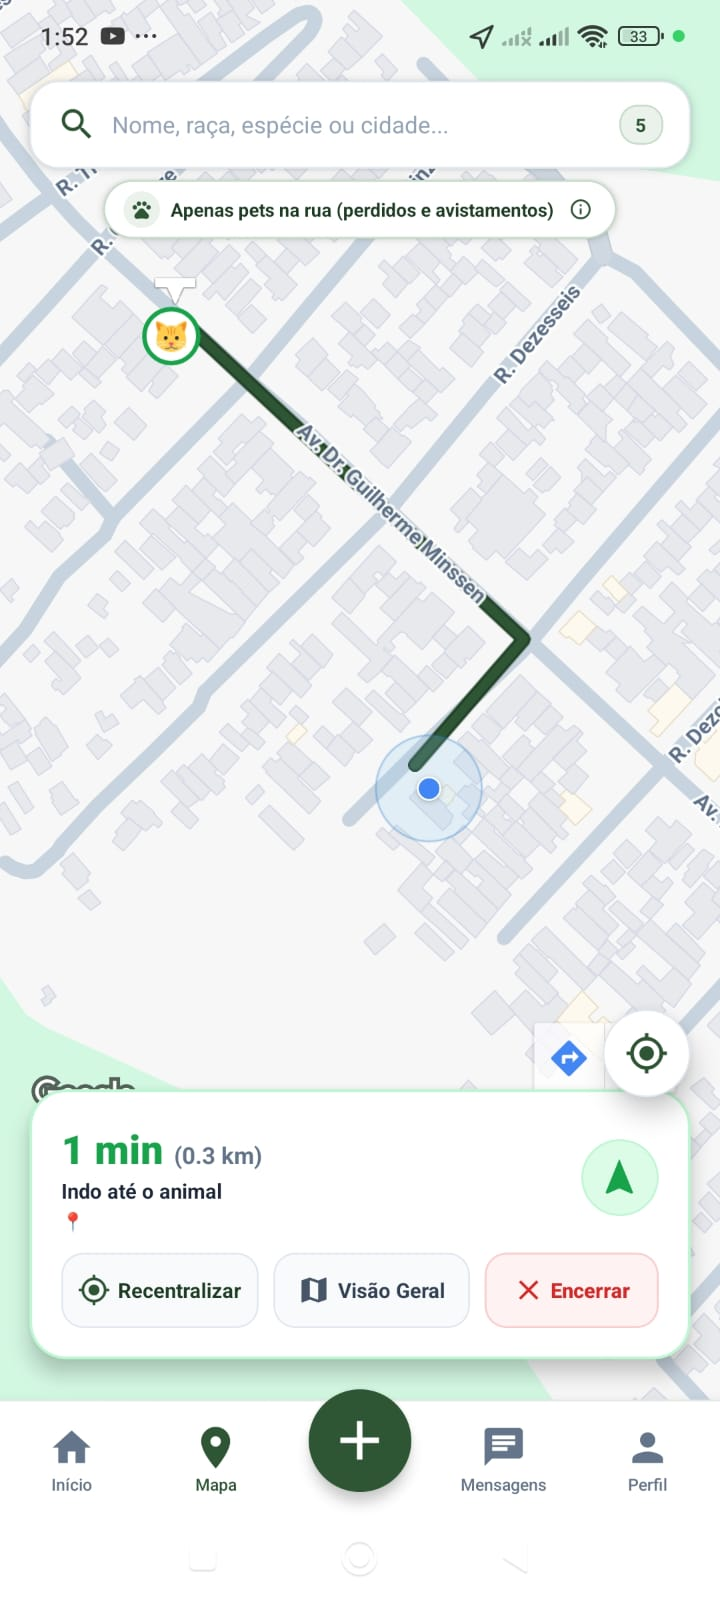
\includegraphics[height=7.8cm, keepaspectratio]{imagens/04_telas_aplicativo/tela-mapa-rota-animal.jpeg}\\[0.15cm]
    \begin{tabular}{p{5.0cm} p{5.0cm}}
        \centering\footnotesize (a) Mapa com Marcadores & \centering\footnotesize (b) Traçado de Rota ao Vivo
    \end{tabular}\\[0.15cm]
    {\footnotesize Fonte: Autoria própria (2026)}
\end{minipage}

\clearpage

\subsection*{Passo 3: Registro de Publicação de Animal Encontrado na Rua}
\noindent
Para cadastrar um animal avistado ou recolhido na rua, o usuário aciona o botão central \textbf{``+''}, define o objetivo do anúncio, anexa fotografias, seleciona os atributos físicos e fixa as coordenadas geográficas exatas no mapa interativo com suporte de geocodificação reversa. A Figura C3 apresenta as etapas de cadastro morfológico e georreferenciamento.

\vspace{0.2cm}
\noindent\begin{minipage}{\linewidth}
\centering
    \textbf{Figura C3: Registro de Publicação e Fixação de Ponto no Mapa}\\[0.2cm]
    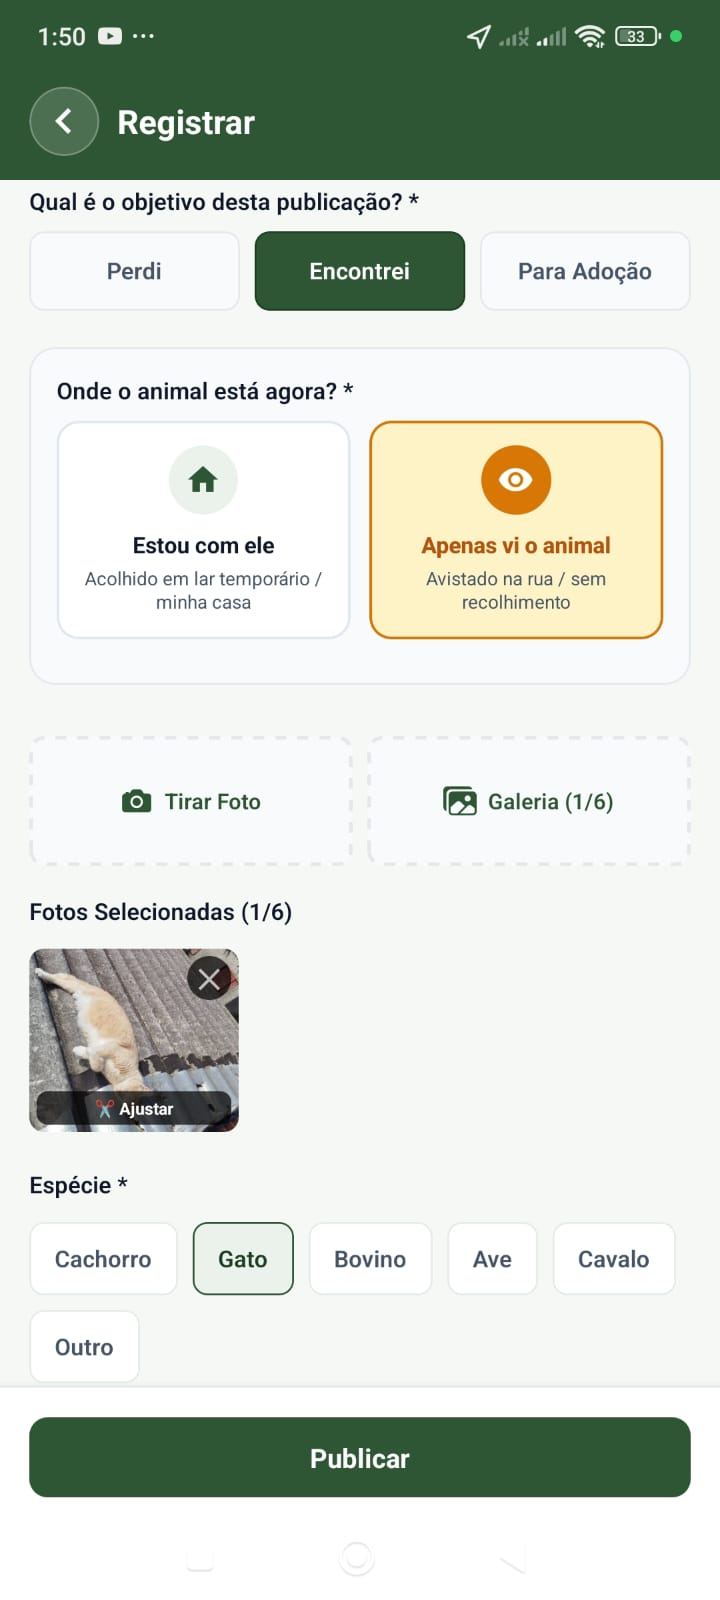
\includegraphics[height=7.8cm, keepaspectratio]{imagens/04_telas_aplicativo/tela-cadastrar-encontrado-1.jpeg}
    \hspace{0.5cm}
    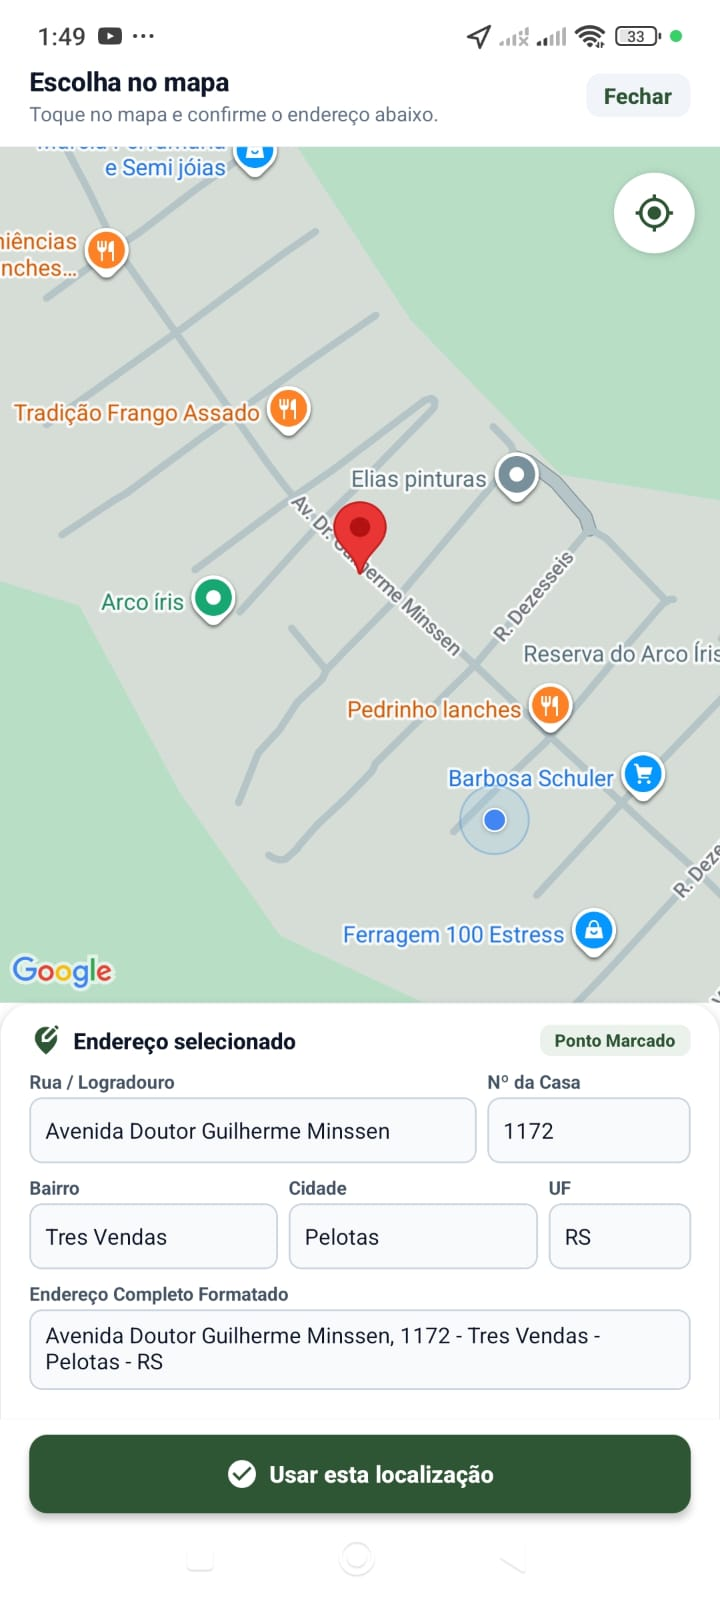
\includegraphics[height=7.8cm, keepaspectratio]{imagens/04_telas_aplicativo/tela-cadastrar-encontrado-3.jpeg}\\[0.15cm]
    \begin{tabular}{p{5.0cm} p{5.0cm}}
        \centering\footnotesize (a) Avistamento e Fotografia & \centering\footnotesize (b) Escolha de Local no Mapa
    \end{tabular}\\[0.15cm]
    {\footnotesize Fonte: Autoria própria (2026)}
\end{minipage}

\clearpage

\subsection*{Passo 4: Consulta de Detalhes e Geração de Cartazes com Código QR}
\noindent
Ao tocar em qualquer animal no feed ou no mapa, a tela de detalhes exibe fotos em alta definição, características físicas e localização aproximada. O tutor pode acionar o botão \textbf{``Compartilhar Cartaz''} para gerar automaticamente cartazes diagramados em múltiplos formatos com código QR integrado. A Figura C4 apresenta a tela de detalhes e o cartaz digital de busca.

\vspace{0.2cm}
\noindent\begin{minipage}{\linewidth}
\centering
    \textbf{Figura C4: Tela de Detalhes do Animal e Cartaz Digital de Busca}\\[0.2cm]
    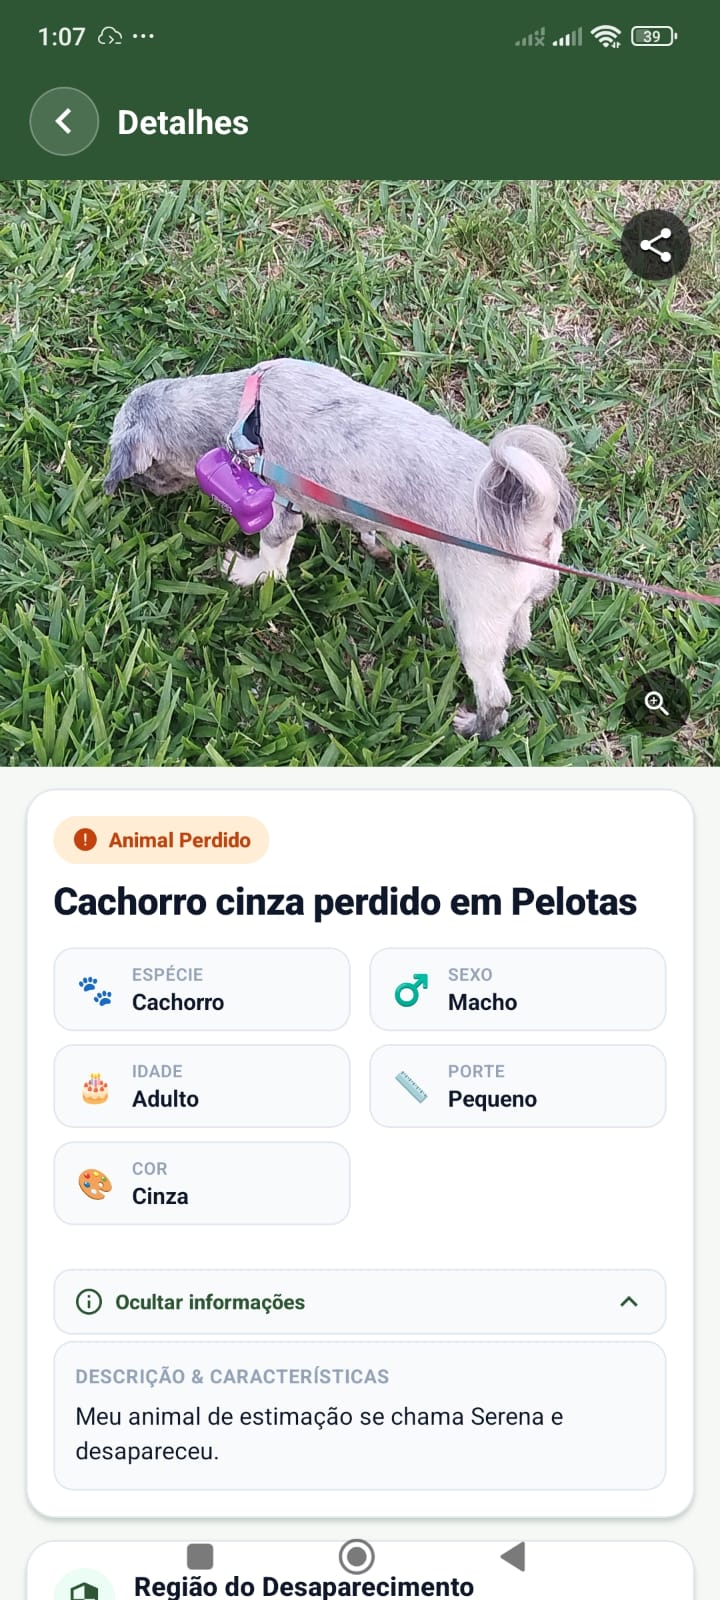
\includegraphics[height=7.8cm, keepaspectratio]{imagens/04_telas_aplicativo/tela-detalhes-do-animal.jpeg}
    \hspace{0.5cm}
    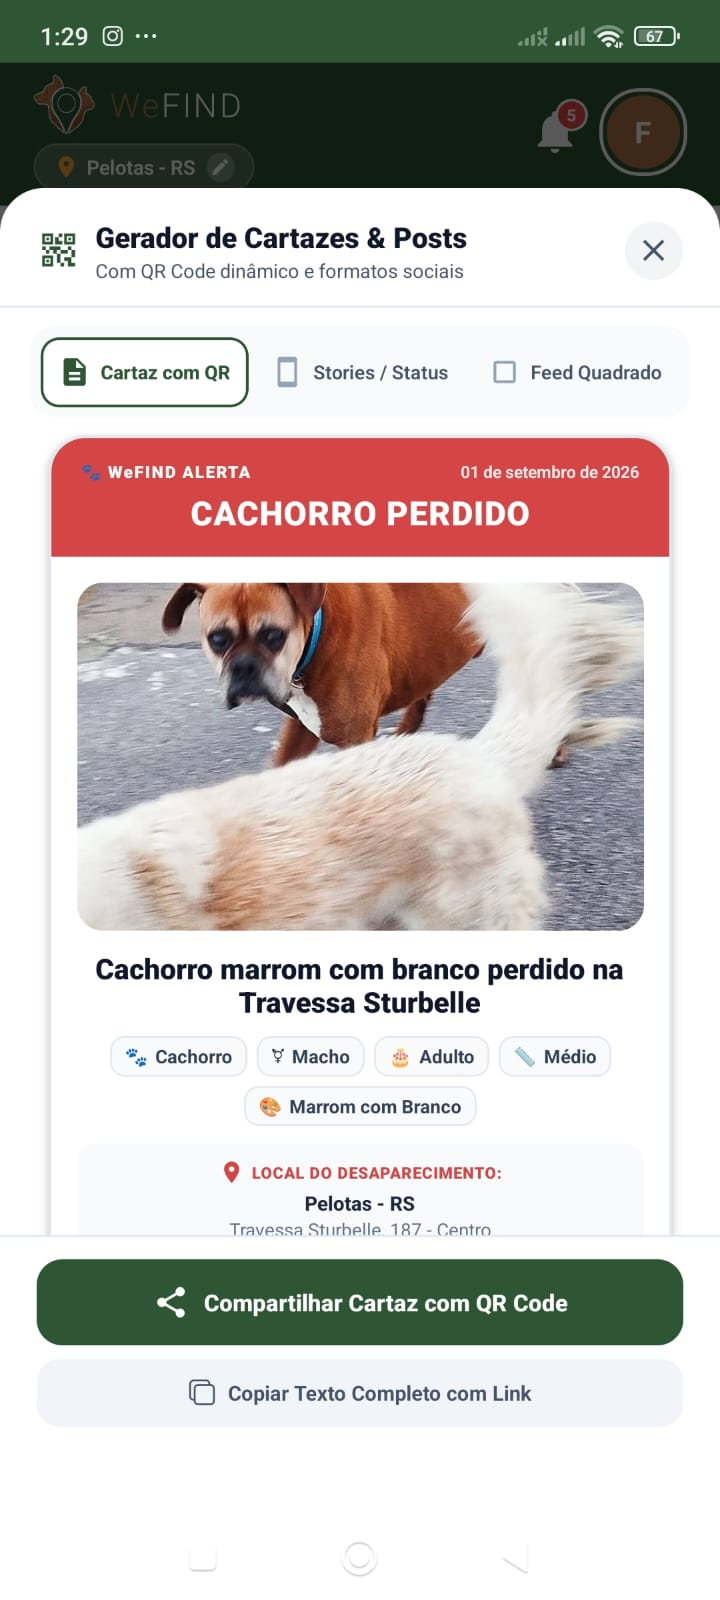
\includegraphics[height=7.8cm, keepaspectratio]{imagens/04_telas_aplicativo/figura21_tela_cartaz.jpeg}\\[0.15cm]
    \begin{tabular}{p{5.0cm} p{5.0cm}}
        \centering\footnotesize (a) Detalhes da Publicação & \centering\footnotesize (b) Cartaz Digital com QR Code
    \end{tabular}\\[0.15cm]
    {\footnotesize Fonte: Autoria própria (2026)}
\end{minipage}

\clearpage

\subsection*{Passo 5: Comunicação Direta e Segura via Chat Interno}
\noindent
Para alinhar o resgate de um animal avistado sem expor números pessoais a fraudes ou trotes, o aplicativo disponibiliza o canal de mensagens privativo em tempo real via WebSockets. A Figura C5 ilustra a caixa de mensagens e a conversa ativa.

\vspace{0.2cm}
\noindent\begin{minipage}{\linewidth}
\centering
    \textbf{Figura C5: Central de Mensagens e Bate-papo Privativo em Tempo Real}\\[0.2cm]
    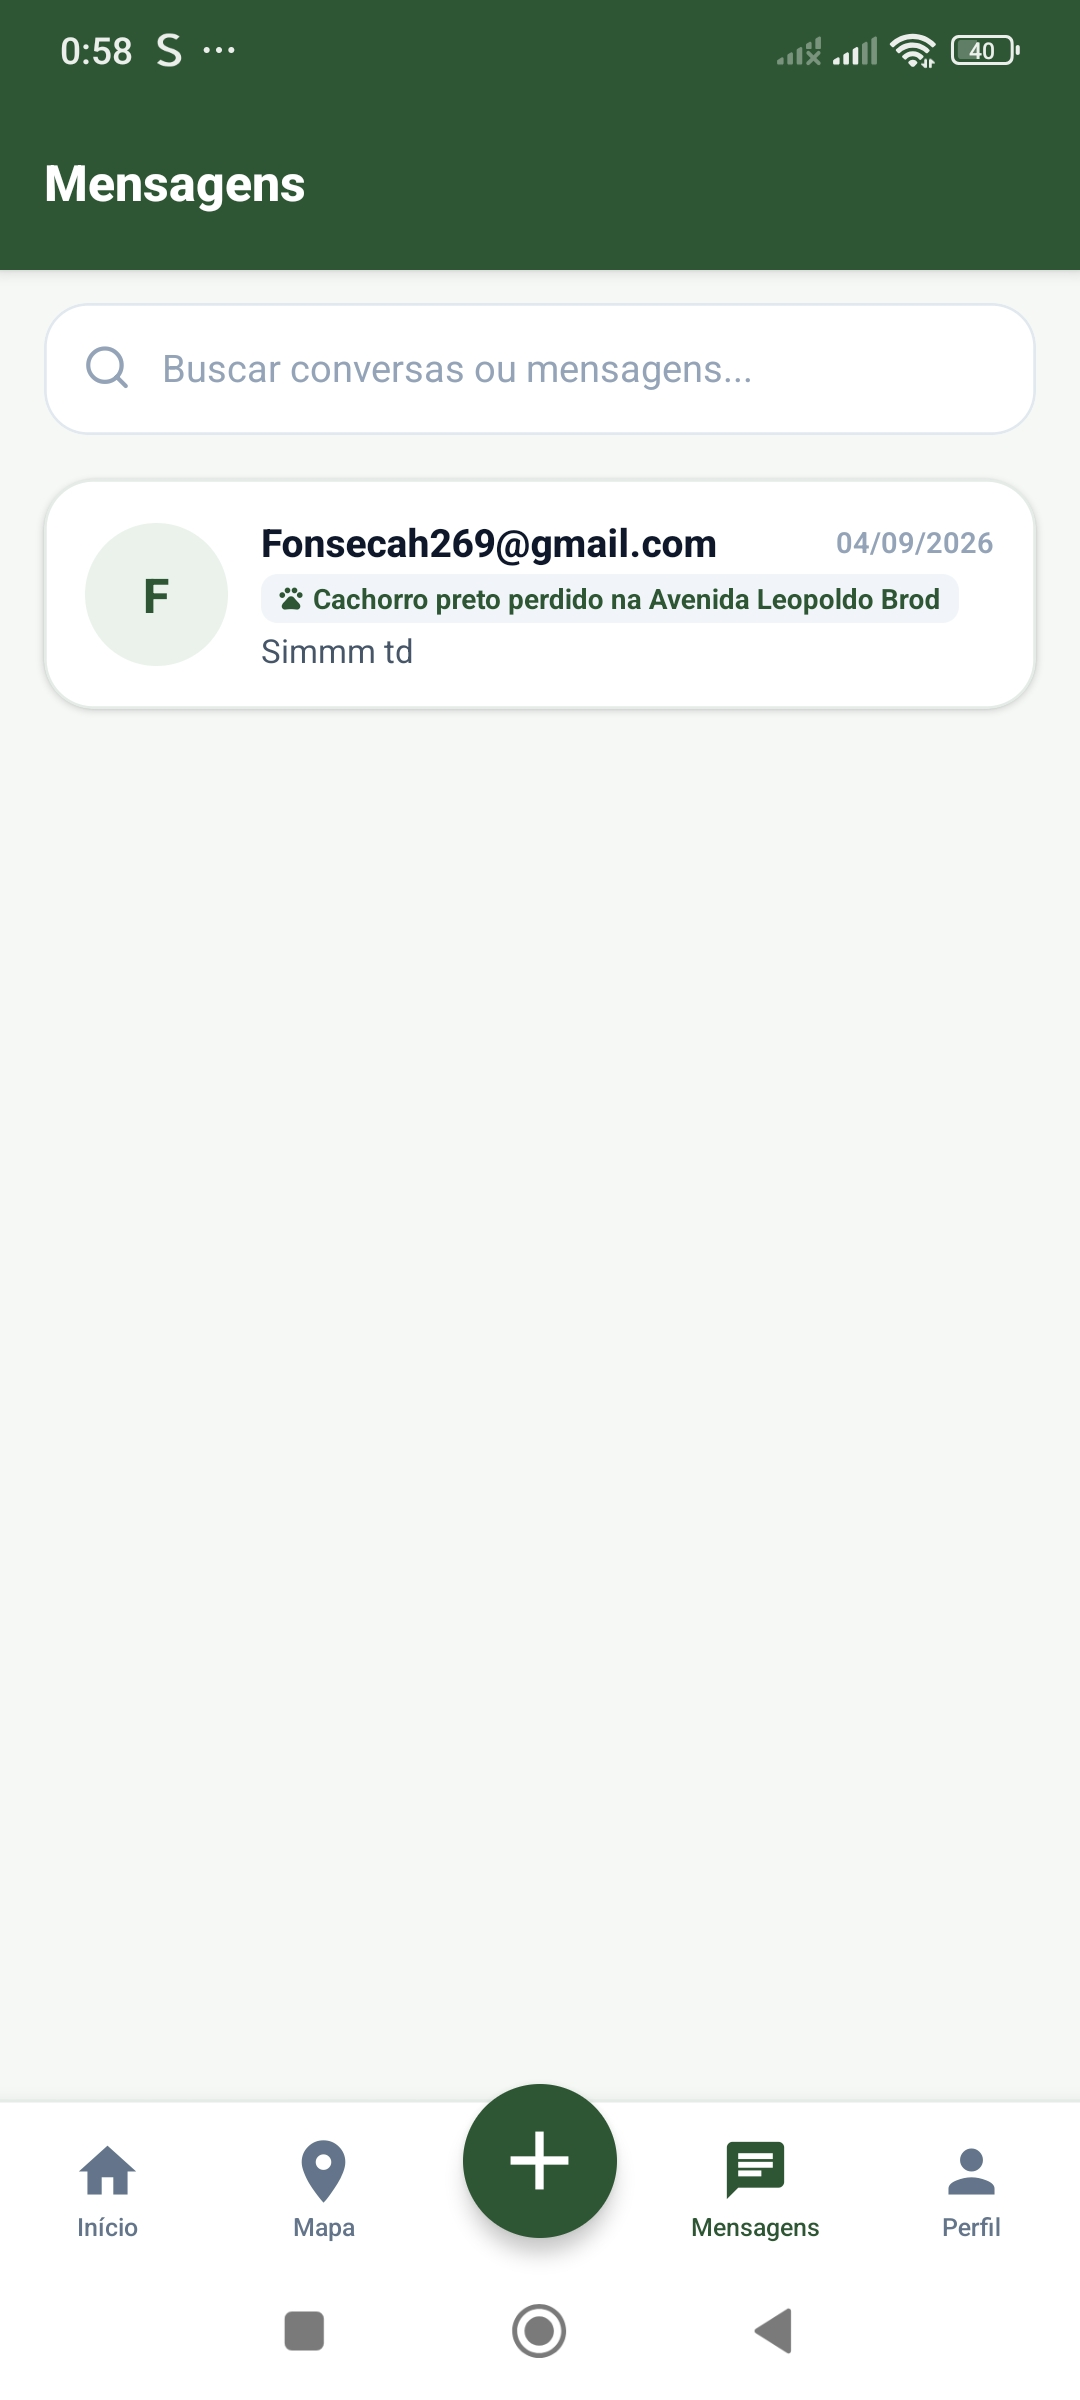
\includegraphics[height=7.8cm, keepaspectratio]{imagens/04_telas_aplicativo/tela-mensagens.jpeg}
    \hspace{0.5cm}
    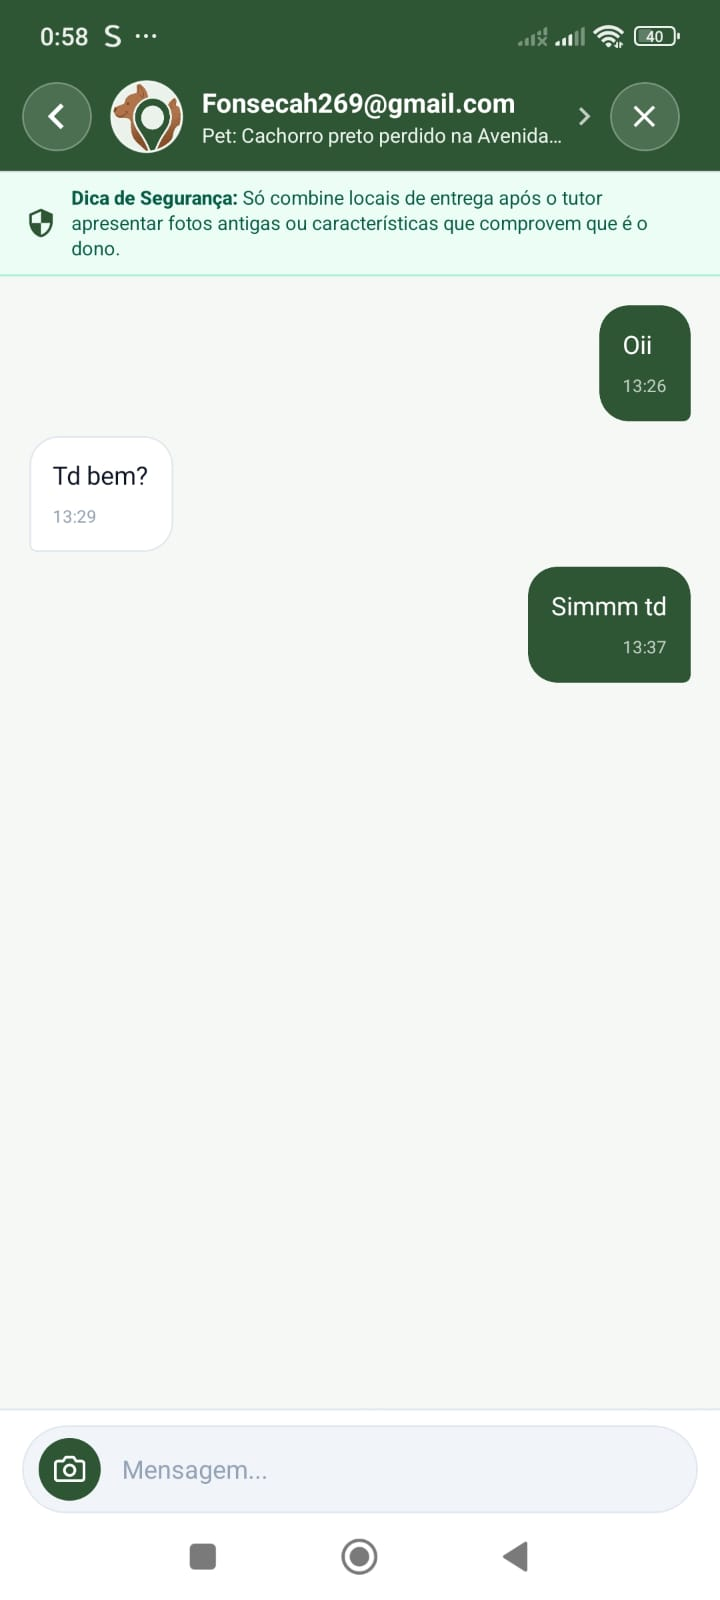
\includegraphics[height=7.8cm, keepaspectratio]{imagens/04_telas_aplicativo/tela-conversa.jpeg}\\[0.15cm]
    \begin{tabular}{p{5.0cm} p{5.0cm}}
        \centering\footnotesize (a) Caixa de Mensagens & \centering\footnotesize (b) Chat em Tempo Real
    \end{tabular}\\[0.15cm]
    {\footnotesize Fonte: Autoria própria (2026)}
\end{minipage}

\clearpage

\subsection*{Passo 6: Cadastro Preventivo e Carteirinha Digital (RG Pet)}
\noindent
Como medida de identificação preventiva, o tutor acessa a área de seus pets no perfil para cadastrar previamente seu animal sob guarda responsável, incluindo vacinas, fotos e marcas singulares. O sistema gera a carteirinha digital de identificação com código QR para identificação rápida em coleiras. A Figura C6 ilustra o painel de gestão preventiva e a carteirinha digital.

\vspace{0.2cm}
\noindent\begin{minipage}{\linewidth}
\centering
    \textbf{Figura C6: Gestão Preventiva de Pets e Carteirinha Digital (RG Pet)}\\[0.2cm]
    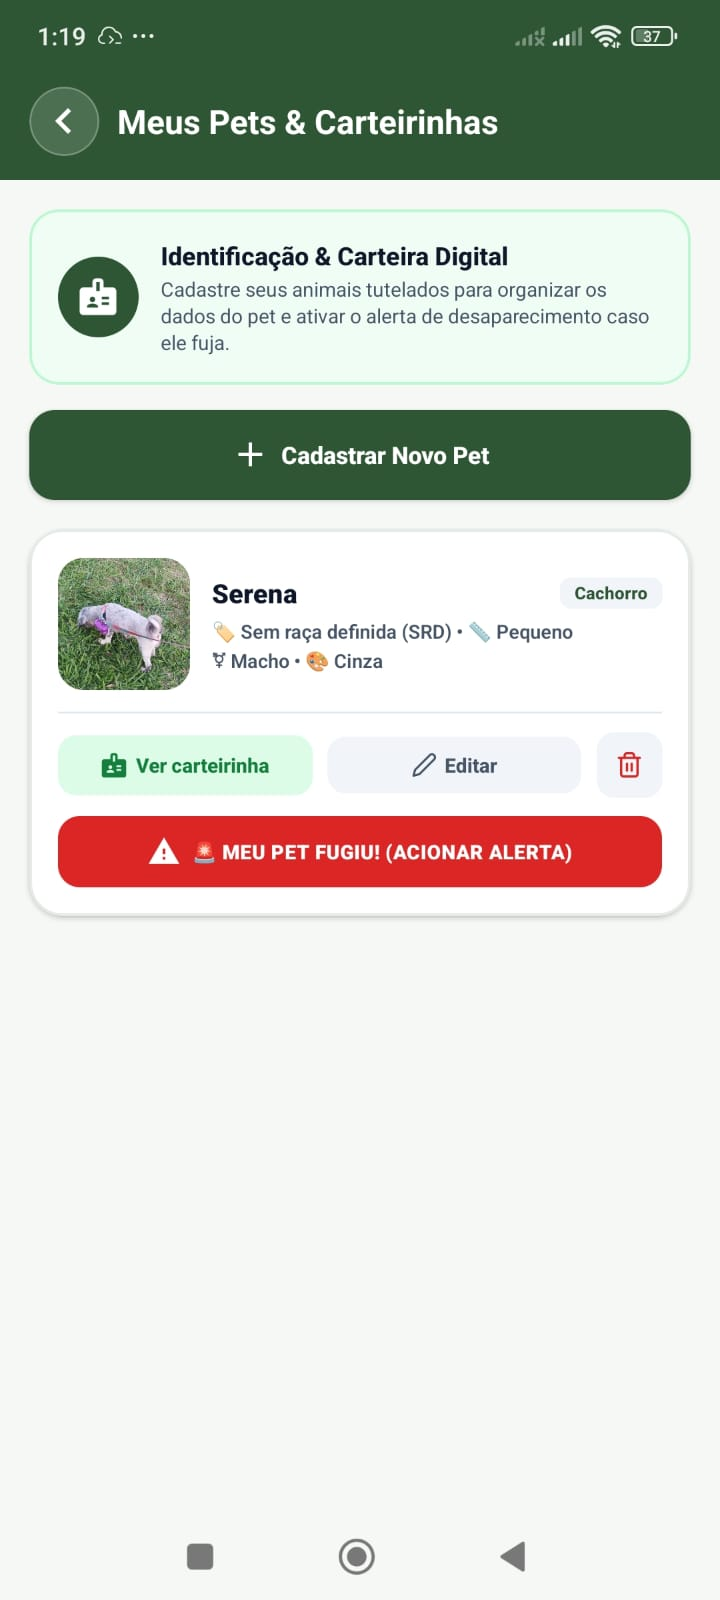
\includegraphics[height=7.8cm, keepaspectratio]{imagens/04_telas_aplicativo/tela-meus-pets-carteirinha-digital.jpeg}
    \hspace{0.5cm}
    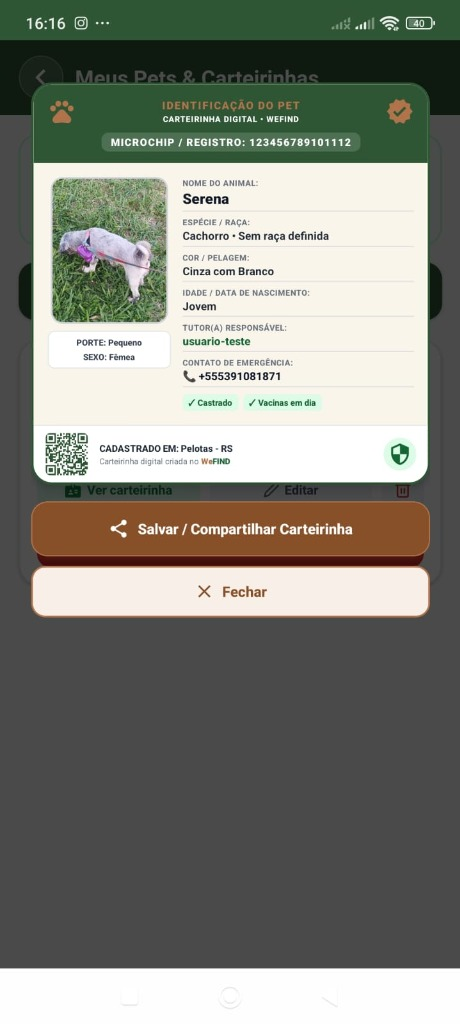
\includegraphics[height=7.8cm, keepaspectratio]{imagens/04_telas_aplicativo/figura25_tela_rg_pet.jpeg}\\[0.15cm]
    \begin{tabular}{p{5.0cm} p{5.0cm}}
        \centering\footnotesize (a) Painel Meus Pets & \centering\footnotesize (b) Carteirinha Digital (RG Pet)
    \end{tabular}\\[0.15cm]
    {\footnotesize Fonte: Autoria própria (2026)}
\end{minipage}

\clearpage